\chapter{Компактное представление результатов исполнения
многопоточной программы}\label{sec:ch4}

\section{Граф состояний}\label{sec:ch2/stategraph}

Как видно из графика~\ref{fig:nds-13-time}, выбор оптимального
алгоритма построения линейных порядков зависит от количества
зависимых пар элементов в частично упорядоченном множестве.
При значениях параметра $p_{D} \lesssim 0.5$ было показано, что учёт
зависимостей обеспечивает существенное преимущество в
производительности по сравнению с учётом независимости.
Поскольку оба подхода (см. алгоритмы~\ref{alg:topo-dep}
и~\ref{alg:topo-indep-lookup}) реализуют построение классов
эквивалентных линейных порядков, выбор конкретного алгоритма
определяется структурой исходного частично упорядоченного множества.
Далее для общности будем обозначать оба алгоритма единым термином —
алгоритм обхода.

Недетерминизм порядка исполнения операций с памятью во время
исполнения многопоточной программы порождает большое количество
возможных состояний многопроцессорной системы.
Ранее было показано, что сложность алгоритмов построения всех
возможных порядков операций с памятью, реализующих все состояния
системы, растёт
экспоненциально~\ref{sec:ch2/topoalg-comp}~\ref{sec:ch2/dep-comp}.
В то же время, рост количества всевозможных состояний так же
экспоненциальный~\ref{sec:ch2/linext-count}.
Тогда в худшем случае верификации всех состояний одной многопоточной
программы необходимо выполнить $2^n$ проверок $2^n$ раз.

Одним из методов упрощения данной задачи является сохранение
результатов алгоритма обхода.
На данный момент сохранение всевозможных результатов исполнения
многопоточной программы поддержано только в
diy7~\ref{sec:litmus-intro} в виде сохранения всех линейных порядков.
В таком случае, для верификации многопоточного теста необходимо
порядка $n \cdot 2^n$ проверок, где $n$ -- количество элементов
линейного порядка, $2^n$ -- количество линейных порядков.

Для оптимизации сохранения всех линейных порядков была разработана
специальная структура данных, позволяющая компактно сохранить
результаты алгоритмов обхода.

Пусть $P = \langle P, <_{p} \rangle$ -- частично упорядоченное
множество, $B$ -- множество всех эквивалентных разбиений, $L_P$ --
множество всех линейных порядков, в котором не существует двух
порядков, принадлежащих одному классу эквивалентности $Eq(\pi, B)$,
$D$ -- множество пар зависимых элементов.

Для элемента $x$ в порядке $\pi \in L_P$ определим:
\begin{itemize}
  \item $V_\pi = \{x\} \cup \{y \mid \#_{\pi}(y) < \#_{\pi}(x),
    \forall y \in \pi,  \}$ -- множество вершин, находящиеся
    ``левее'' элемента $x$;
  \item $E_\pi = \{(b, a) \mid \{a, b\} \in D \text{ или } a <_p b,
    \text{ где } \#_{\pi}(a) < \#_{\pi}(b), \forall a,b \in V_\pi \}$
    -- множество направленных рёбер ``справа налево'' между
    зависимыми элементами или элементами с отношением порядка.
\end{itemize}
По построению граф $G_\pi = (V_\pi, E_\pi)$ является ориентированным
и ацикличным.
В таком графе для элемента $x$ существуют простые цепи (без циклов),
в которых все вершины и рёбра различны~\cite{graph-theory}.

\begin{definition}
  \textbf{Путём} $\rho$ элемента $x$ для порядка $\pi$ назовём
  подпорядок, из элементов $Y \subseteq \pi$, для которых существует
  простая цепь из $x$ в $\forall y \in Y$.
  \begin{equation}
    \begin{multlined}
      \rho = \{y \in \pi \mid \exists (x, y) \text{ -- простая цепь
      от вершины } x \text{ в вершину } y \} \\
      \text{ и относительный порядок элементов в } \rho \text{ такой
      же, как в } \alpha
    \end{multlined}
    \label{eq:def_suborder}
  \end{equation}
  и обознаячается $\rho_{\pi}(x)$.
\end{definition}

Иными словами, $\rho_{\pi}(x)$ можно интерпретировать как порядок
только тех операций, от которых зависит состояние операции $x$.

Различные $\rho_{\pi}(x)$ на примере частично упорядоченного
множества, как на рисунке~\ref{fig:topo-dep}, продемонстрированы в
таблице~\ref{tab:rho_exam}.

\begin{table}[ht]
  \caption{$\rho_{\pi}(x)$ для частично упорядоченного
  множества~\ref{fig:topo-dep}.}
  \centering
  \begin{tabular}{llllll}
    Линейный порядок $\pi$ & $\rho_{\pi}(0)$ & $\rho_{\pi}(1)$ &
    $\rho_{\pi}(2)$ & $\rho_{\pi}(3)$ & $\rho_{\pi}(4)$ \\
    $\alpha = 04123$ & 0 & 01 & 012 & 0123 & 04 \\
    $\beta = 04132$ & 0 & 01 & 0132 & 013 & 04 \\
    $\gamma = 40123$ & 40 & 401 & 4012 & 40123 & 4 \\
    $\zeta = 40132$ & 40 & 401 & 40132 & 4013 & 4
  \end{tabular}
  \label{tab:rho_exam}
\end{table}

В таблице видно, что $\rho_{\alpha}(0) = \rho_{\beta}(0)$,
$\rho_{\gamma}(0) = \rho_{\zeta}(0)$, $\rho_{\alpha}(1) =
\rho_{\beta}(1)$, $\rho_{\gamma}(1) = \rho_{\zeta}(1)$,
$\rho_{\alpha}(4) = \rho_{\beta}(4)$ и $\rho_{\gamma}(4) = \rho_{\zeta}(4)$.
Всего существует 14 уникальных путей от каждой вершины для всех
линейных порядков.

\begin{definition}
  \textbf{Графом состояний} SG(state graph) -- называется
  ориентированный граф, построенный по правилу~\ref{eq:sg_def}.

  \begin{equation}
    \begin {aligned}
    &V_{SG} = \{ \rho_{\pi}(x) \mid (x, \pi) \in P \times L_P \} \\
    &E_{SG} = \{ (\rho_{\pi}(x), \rho_{\pi}(y)) \mid (x, y) \in
    E_\pi, \forall \pi \in L_P, \forall x, y \in P \} \\
    &SG = (V_{SG}, E_{SG})
    \end {aligned}
    \label{eq:sg_def}
    \end {equation}
  \end{definition}

  На рисунке~\ref{fig:sg-topo-dep} изображён граф состояния для
  примера~\ref{fig:topo-dep}.
  Для простоты здесь и далее будем изображать рёбра графа только с
  отношением ближайшего соседства.
  Также истоки графа изображены снизу, потому что исток отражает путь
  максимальной длины для данного подпорядка.

  \begin{figure}[htbp]
    \centerfloat{
      \begin{tikzpicture}[
    node distance=1.5cm and 1cm,
    dag/.style={circle, draw=black, fill=white, inner sep=2pt, minimum size=8mm},
    order/.style={stealth-, thick},
]
\begin{scope}[xshift=-3cm]
\node[dag] (0_0) {$\rho_{\alpha}(0)$};
\node[dag, below left=0.5cm of 0_0] (4_1) {$\rho_{\alpha}(4)$};
\node[dag, right=1.0cm of 4_1] (1_1) {$\rho_{\alpha}(1)$};
\node[dag, below left=0.5cm of 1_1] (2_2) {$\rho_{\alpha}(2)$};
\node[dag, right=1.0cm of 2_2] (3_2) {$\rho_{\beta}(3)$};
\node[dag, below=0.5cm of 3_2] (2_3) {$\rho_{\beta}(2)$};
\node[dag, below=0.5cm of 2_2] (3_3) {$\rho_{\alpha}(3)$};

\draw[order] (0_0) -- (4_1);
\draw[order] (0_0) -- (1_1);
\draw[order] (1_1) -- (2_2);
\draw[order] (2_2) -- (3_3);
\draw[order] (1_1) -- (3_2);
\draw[order] (3_2) -- (2_3);
\end{scope}

\begin{scope}[xshift=3cm]
\node[dag] (4_0) {$\rho_{\gamma}(4)$};
\node[dag, below=0.5cm of 4_0] (0_1) {$\rho_{\gamma}(0)$};
\node[dag, below=0.5cm of 0_1] (1_2) {$\rho_{\gamma}(1)$};
\node[dag, below left=0.5cm of 1_2] (2_3) {$\rho_{\gamma}(2)$};
\node[dag, right=1.0cm of 2_3] (3_3) {$\rho_{\zeta}(3)$};
\node[dag, below=0.5cm of 3_3] (2_4) {$\rho_{\zeta}(2)$};
\node[dag, below=0.5cm of 2_3] (3_4) {$\rho_{\gamma}(3)$};


\draw[order] (4_0) -- (0_1);
\draw[order] (0_1) -- (1_2);
\draw[order] (1_2) -- (2_3);
\draw[order] (2_3) -- (3_4);
\draw[order] (1_2) -- (3_3);
\draw[order] (3_3) -- (2_4);
\end{scope}

\end{tikzpicture}

    }
    \caption{Граф состояний для примера~\ref{fig:topo-dep}.}
    \label{fig:sg-topo-dep}
  \end{figure}

  По построению графа состояний в вершине $\rho_{\pi}(x)$ нет
  необходимости хранить сам подпорядок, так как его можно
  восстановить алгоритмом~\ref{alg:bfs_sg} обхода в ширину от вершины
  $x$ по графу состояний.

  \begin{algorithm}[H]
    \caption{Построение пути по графу состояний}
    \label{alg:bfs_sg}
    \begin{algorithmic}[1]
      \Require
      $SG(V, E)$ -- граф состояний.
      $x$ -- вершина графа состояния,
      \Ensure $\rho$ -- путь.
      \Function{bfs}{$x$}

      \State $queue \gets$ пустая очередь
      \State $\rho \gets$ пустой список

      \State $visited = \{x\}$
      \State $queue.\text{push}(x)$

      \While{$queue$ не пуста}
      \State $u \gets queue.\text{front}()$
      \State $queue.\text{pop}()$
      \State $\rho.\text{push\_front}(u)$

      \For{$(u, v) \in E$}
      \If{$v \not \in visited$}
      \State $visited \gets visited \cup v$
      \State $queue.\text{push}(v)$
      \EndIf
      \EndFor
      \EndWhile

      \State \Return $\rho$
      \EndFunction
    \end{algorithmic}
  \end{algorithm}

  \begin{lemma}
    Любые два различных $\pi, \tau \in V_{SG}$, состоящие из одних
    элементов, принадлежат разным классам эквивалентности.
    \label{lm:path-unique}
  \end{lemma}

  \begin{proof}
    Докажем от противного. \\
    Пусть $\exists \pi,\tau \in V_{SG}$ такие, что $\pi \in Eq(\tau, B)$.
    То есть, $\pi$ может быть получено из $\tau$ перестановкой
    элементов из разбиения $B$.
    Тогда:
    \begin{subequations}
      \begin{align}
        &\exists \{ab,ba\} \in B \mid ab \in \pi, ba \in \tau \text{
        и выполняется } \label{eq:diff_order1} \\
        &\#_{\pi}(a) < \#_{\pi}(b) \text{ и } \#_{\tau}(b) <
        \#_{\tau}(a) \label{eq:diff_order2}
      \end{align}
      \label{eq:diff_order}
    \end{subequations}
    Из условия~\ref{eq:diff_order1} следует, что элементы $a,b \not
    \in D$. Из условия~\ref{eq:diff_order2} следует, что между
    элементами $a,b$ нет отношения порядка.

    Пусть $b$ -- это последняя вершина в порядке $\pi$.
    Тогда вершина $a$ недостижима из вершины $b$, так как между ними
    нет отношения порядка или зависимости.
    Следовательно (см.~\ref{eq:def_suborder}~\ref{eq:sg_def}), $a \not \in \pi$.
    Аналогичные рассуждения верны для $b$ в $\tau$, поэтому пути
    $\pi,\tau$ не могут начинаться с вершин $a, b$.

    Пусть $\exists c$ такое, что $a,b$ достижимы и в пути $\pi$, и в
    пути $\tau$ из вершины $c$.
    Достроим пути $\pi, \tau$ до линейных порядков частично
    упорядоченного множества, сохраняя относительный порядок
    добавленных элементов:
    $\alpha \in L_P \mid \pi = \rho_\alpha(c)$, $\beta \in L_P \mid
    \tau = \rho_\beta(c)$.
    Тогда $\alpha$ может быть получен из $\beta$ перестановкой только
    элементов $\{ab, ba\}$, следовательно $\alpha \in Eq(\beta, B)$,
    что противоречит заданию множества всех линейных порядков $L_P$.

  \end{proof}

  \subsection{Граф состояния многопоточной программы}

  Как было указано выше, элементами частично упорядоченного множества
  $P$ являются операции с памятью.
  Все операции с памятью, которые изменяют состояние регистров,
  обозначим $R$, то есть операции чтения или чтения-модификации-записи.
  Другие операции (записи, барьера), обозначим $W$.
  Множество $D$ состоит из попарно зависимых операций с памятью.
  Если переупорядочить эти операции, то система будет приведена в
  иное состояние.

  Таким образом, вершина графа состояний отображает состояние системы
  в момент исполнения соответствующей операции и порядок операций,
  которые привели систему в данное состояние.

  \subsection{Верификация по графу состояния}

  Так как любые два истока графа состояния принадлежат разным классам
  эквивалентности (см.~\ref{lm:path-unique}), а класс эквивалентности
  соответствует уникальному состоянию системы, то любой исток графа
  состояния соответствует уникальному состоянию системы.
  Поэтому построенный граф состояний можно эффективно использовать
  для проверки корректности исполнения многопоточной программы на
  многопроцессорной системе.
  Для начала, дополним каждые вершины графа, соответствующие операции
  чтения $R$, информацией об значениях, прочитанных данной операцией
  с памятью в данном порядке.

  Определим операцию получения элемента частично упорядоченного
  множества из вершины графа состояний следующим образом:
  \begin{equation}
    \forall \rho_{\pi}(x) \in V_{SG} \; \exists! x \in P \; \text{
    такой, что } \; x = op(\rho_{\pi}(x))
    \label{eq:op_rho}
  \end{equation}

  Вершина графа состояний соответствует состоянию системы
  $reg_{\alpha}(x) \equiv reg(\rho_{\alpha}(x))$.
  Так как никакая операция $W$ не изменяет регистры, то $\forall x
  \in W, \forall \alpha,\beta \in L_P \ \rightarrow reg_{\alpha}(x) =
  reg_{\beta}(x)$.
  Аналогично для операций $F$.

  \begin{definition}
    \label{def:mark}
    Во время исполнения многопоточной программы операциям с памятью
    ставится в соответствие значение, прочитанное данной операцией с памятью.
    Эти значения отражаются на графе состояний с помощью
    \textbf{маркированных} вершин графа: $\mathcal{M} =
    \{\rho_{\alpha}(x) \in V_{SG} \mid reg_{\alpha}(x) \in trace \}$.
  \end{definition}

  \textbf{Первое условие корректности} исполнения многопоточной
  программы: все операции с памятью в многопоточной программе промаркированы.
  \begin{equation}
    \label{eq:verif-1st}
    \forall x \in P \; \exists \alpha \in L_P \rightarrow
    \rho_{\alpha}(x) \in \mathcal{M}
  \end{equation}
  Если существует операция, для которой нет вершины в графе
  состояния, то исполнение этой операции привело к ошибке, не
  связанной с моделью памяти.

  \textbf{Второе условие корректности} исполнения многопоточной
  программы: существует множество путей из истоков графа состояния,
  покрывающее все маркированные вершины графа.
  \begin{align}
    \label{eq:verif-2nd}
    & visited = \{\text{bfs}(l) \mid \forall l \text{ -- исток },
      \forall \rho \in \text{bfs}(l) \rightarrow \rho \in \mathcal{M}
    \} \nonumber \\
    & \text{Исполнение программы корректно, если } op(visited) = P
  \end{align}
  Выполнение этого условия обеспечивает соответствие исполнения
  многопоточной программы заданной модели памяти.

  \begin{lemma}
    Из условия корректности верификации по графу состояний
    \ref{eq:verif-1st} и \ref{eq:verif-2nd}(1) следует условие
    корректности верификации по линейным порядкам~\ref{eq:verif-base}(2).
    \label{lm:verif-equals}
  \end{lemma}

  \begin{proof}

    $\forall x \in P \rightarrow \exists \rho_{\alpha}(x) \in
    visited$. Это всегда можно сделать из условия~\ref{eq:verif-2nd}.
    Выберем такие $src = \{\rho_{\alpha}(x) \mid \rho_{\alpha}(x)
    \text{ -- исток}\}$.
    Тогда построим линейный порядок следующим образом:

    \begin{algorithm}[H]
      \caption{Построение линейного порядка из множества истоков
      графа состояния}
      \label{alg:linext-from-leaf}
      \begin{algorithmic}[1]
        \Require $src$ -- истоки. $SG$ -- граф состояния.
        \Ensure $\pi$ -- линейный порядок.
        \Function{ConstructLinext}{$src$, $SG$}
        \State $\pi \gets \text{пустой порядок}$
        \ForAll{$l \in src$}
        \State $ops \gets ( op(\rho) \mid \rho \in  \mathcal{M},
        \forall \rho \in \text{bfs}(l))$ \Comment $\forall x \in ops
        \rightarrow reg(x) \in trace$ из условия~\ref{eq:verif-1st}
        \ForAll{$x \in ops \mid x \not \in \pi$}
        \State $\pi\text{.add\_front}(x)$
        \EndFor
        \EndFor

        \State \Return $\pi$
        \EndFunction
      \end{algorithmic}
    \end{algorithm}

    Порядок, построенный по алгоритму~\ref{alg:linext-from-leaf}
    всегда состоит из операций, которые соответствуют состоянию
    программы (условие~\ref{eq:verif-1st}).
    Порядок операций сохранён относительно начального частично
    упорядоченного множества программы, так как граф состояния
    сохраняет относительный порядок операций.
    И в построенном порядке присутствуют все элементы частично
    упорядоченного множества, из условия~\ref{eq:verif-2nd}.

    Таким образом, найден линейный порядок $\pi$, удовлетворяющий
    условию~\ref{eq:verif-base}.

  \end{proof}

  \subsection{Пример}

  \fixme{this already has been printed. ~\ref{fig:litmus-ex}}

  Рассмотрим подробнее использование графа состояний на примере
  литмус-теста~\ref{fig:litmus-ex}.

  \begin{minipage}[ht]{\textwidth}
    \centering
    \lstinputlisting[caption={Пример литмуса},
    label={fig:litmus-ex-copy}, captionpos=b]{src/litmus-example.txt}
  \end{minipage}

  Обозначим:
  $\text{W}_y = \texttt{MOV [y],\$1}$,
  $\text{R}_x = \texttt{MOV EAX,[x]}$,
  $\text{W}_x = \texttt{MOV [x],\$1}$,
  $\text{R}_y = \texttt{MOV EAX,[y]}$,

  \begin{figure}[ht]
    \begin{subfigure}[b]{0.5\textwidth}
      \centering
      \input{Dissertation/images/litmus-SC.tex}
      \caption{Частично упорядоченное множество для SC модели памяти}
      \label{fig:litmus-sc-program-graph}
    \end{subfigure}%
    \begin{subfigure}[b]{0.5\textwidth}
      \centering
      \begin{tikzpicture}[
    node distance=1.5cm and 1.5cm,
    >=Stealth,
    every node/.style={on grid, rectangle, draw, minimum size=8mm}
]

% Define nodes
\node (Wy) {$\text{W}_y$};
\node[below=of Wy] (Rx) {$\text{R}_x$};

\node[right=of Wy] (Wx) {$\text{W}_x$};
\node[below=of Wx] (Ry) {$\text{R}_y$};

\draw[black, dashed, ->] (Wx) -- (Ry);
\draw[black, dashed, ->] (Wy) -- (Rx);

\draw[black, dashed, -] (Wx) -- (Rx);
\draw[black, dashed, -] (Wy) -- (Ry);

\end{tikzpicture}

      \caption{Частично упорядоченное множество для TSO модели памяти}
      \label{fig:litmus-tso-program-graph}
    \end{subfigure}
    \caption{Частично упорядоченные множества для
    литмус-теста~\ref{fig:litmus-ex}}
    \label{fig:litmus-program-graph}
  \end{figure}

  На рисунках~\ref{fig:litmus-program-graph} представлены частично
  упорядоченные множества для двух различных моделей памяти:
  слева для SC~\ref{fig:litmus-sc-program-graph},
  справа для TSO~\ref{fig:litmus-tso-program-graph}.
  Красное направленное ребро обозначает PPO-порядок, пунктирное
  направленное -- PO, пунктирное ненаправленное -- зависимости операций.
  SC-модель памяти отличается от TSO тем, что эффект операций $W$,
  $R$ в памяти может быть наблюдаем в другом порядке.

  Различные $\rho_{\pi}(x)$ для SC-модели
  памяти~\ref{fig:litmus-sc-program-graph} и граф состояний
  продемонстрированы в таблице~\ref{tab:litmus-sc-rho} и на
  рисунке~\ref{fig:sg-litmus-sc}.

  \begin{table}[ht]
    \caption{$\rho_{\pi}(x)$ для частично упорядоченного
    множества~\ref{fig:litmus-sc-program-graph}.}
    \centering
    \begin{tabular}{llllll}
      Линейный порядок $\pi$ & $\rho_{\pi}(\text{W}_x)$ &
      $\rho_{\pi}(\text{W}_y)$ & $\rho_{\pi}(\text{R}_x)$ &
      $\rho_{\pi}(\text{R}_y)$ \\
      $\alpha = \text{W}_x \text{R}_y \text{W}_y \text{R}_x$ &
      $\text{W}_x$ & $\text{W}_x \text{R}_y \text{W}_y $ &
      $\text{W}_x \text{R}_y \text{W}_y \text{R}_x$ & $\text{W}_x
      \text{R}_y $ \\
      $\beta = \text{W}_x \text{W}_y \text{R}_x \text{R}_y$ &
      $\text{W}_x $ & $\text{W}_y$ & $\text{W}_x \text{W}_y
      \text{R}_x$ & $\text{W}_x \text{W}_y \text{R}_y$ \\
      $\gamma = \text{W}_y \text{R}_x \text{W}_x \text{R}_y$ &
      $\text{W}_y \text{R}_x \text{W}_x $ & $\text{W}_y $ &
      $\text{W}_y \text{R}_x $ & $\text{W}_y \text{R}_x \text{W}_x \text{R}_y$
    \end{tabular}
    \label{tab:litmus-sc-rho}
  \end{table}

  \begin{figure}[ht]
    \centerfloat{
      
\begin{tikzpicture}[
    node distance=1.5cm and 1cm,
    dag/.style={circle, draw=black, fill=white, inner sep=2pt, minimum size=20mm, align=center},
    order/.style={stealth-, thick},
]
\node[dag] (1) {$W_x$};
\node[dag, right=1.0cm of 1] (2) {$W_y$};

\node[dag, below=1.0cm of 1] (4) {$R_x$\\EAX=1};
\node[dag, left=1.0cm of 4] (3) {$R_y$\\EAX=0};
\node[dag, below=1.0cm of 2] (5) {$R_y$\\EAX=1};
\node[dag, right=1.0cm of 5] (6) {$R_x$\\EAX=0};

\node[dag, below=1.0cm of 3] (7) {$W_y$};
\node[dag, below=1.0cm of 7] (8) {$R_x$\\EAX=1};

\node[dag, below=1.0cm of 6] (9) {$W_x$};
\node[dag, below=1.0cm of 9] (10) {$R_y$\\EAX=1};

\draw[order] (1) -- (3);
\draw[order] (1) -- (4);
\draw[order] (1) -- (5);

\draw[order] (2) -- (4);
\draw[order] (2) -- (5);
\draw[order] (2) -- (6);

\draw[order] (3) -- (7);
\draw[order] (7) -- (8);

\draw[order] (6) -- (9);
\draw[order] (9) -- (10);


\end{tikzpicture}

    }
    \caption{Граф состояний теста~\ref{fig:litmus-ex} для SC-модели памяти.}
    \label{fig:sg-litmus-sc}
  \end{figure}

  Различные $\rho_{\pi}(x)$ для TSO-модели
  памяти~\ref{fig:litmus-tso-program-graph} и граф состояний
  продемонстрированы в таблице~\ref{tab:litmus-tso-rho} и на
  рисунке~\ref{fig:sg-litmus-tso}.

  \begin{table}[ht]
    \caption{$\rho_{\pi}(x)$ для частично упорядоченного
    множества~\ref{fig:litmus-tso-program-graph}.}
    \centering
    \begin{tabular}{llllll}
      Линейный порядок $\pi$ & $\rho_{\pi}(\text{W}_x)$ &
      $\rho_{\pi}(\text{W}_y)$ & $\rho_{\pi}(\text{R}_x)$ &
      $\rho_{\pi}(\text{R}_y)$ \\
      $\alpha = \text{W}_x \text{R}_y \text{W}_y \text{R}_x$ &
      $\text{W}_x$ & $\text{R}_y \text{W}_y$ & $\text{W}_x
      \text{R}_x$ & $\text{R}_y $ \\
      $\beta = \text{W}_x \text{W}_y \text{R}_x \text{R}_y$ &
      $\text{W}_x $ & $\text{W}_y$ & $\text{W}_x \text{R}_x$ &
      $\text{W}_y \text{R}_y$ \\
      $\gamma = \text{W}_y \text{R}_x \text{W}_x \text{R}_y$ &
      $\text{R}_x \text{W}_x $ & $\text{W}_y $ & $\text{R}_x$ &
      $\text{W}_y \text{R}_y$ \\
      $\zeta = \text{R}_x \text{R}_y \text{W}_x \text{W}_y$ &
      $\text{R}_x \text{W}_x $ & $\text{R}_y \text{W}_y $ &
      $\text{R}_x$ & $\text{R}_y$

    \end{tabular}
    \label{tab:litmus-tso-rho}
  \end{table}

  \begin{figure}[ht]
    \centerfloat{
      
\begin{tikzpicture}[
    node distance=1.5cm and 1cm,
    dag/.style={circle, draw=black, fill=white, inner sep=2pt,
    minimum size=20mm, align=center},
    order/.style={stealth-, thick},
  ]
  \node[dag] (1) {$W_x$};
  \node[dag, right=1.0cm of 1] (2) {$R_x$\\EAX=0};
  \node[dag, right=1.0cm of 2] (3) {$W_y$};
  \node[dag, right=1.0cm of 3] (4) {$R_y$\\EAX=0};

  \node[dag, below=1.0cm of 1] (5) {$R_x$\\EAX=1};
  \node[dag, below=1.0cm of 2] (6) {$W_x$};
  \node[dag, below=1.0cm of 3] (7) {$R_y$\\EAX=1};
  \node[dag, below=1.0cm of 4] (8) {$W_y$};

  \draw[order] (1) -- (5);
  \draw[order] (2) -- (6);
  \draw[order] (3) -- (7);
  \draw[order] (4) -- (8);

\end{tikzpicture}

    }
    \caption{Граф состояний теста~\ref{fig:litmus-ex} для TSO-модели памяти.}
    \label{fig:sg-litmus-tso}
  \end{figure}

  Граф состояний хранит в себе информацию о всех возможных эффектах в
  памяти, а также информацию о порядке исполнения операций, который
  приводит к этим эффектам в памяти.

  Пусть каждой операции с памятью в многопоточной программе
  соответствует состояние памяти для каждого возможного линейного
  порядка операций.
  Множества $S_{linext} = \{reg_{\alpha}(x) \mid \forall x \in P,
  \forall \alpha \in L(P)\}$ определяют все возможные состояния
  памяти многопоточной программы.
  Размер этого множества считается по формуле~\ref{eq:linext-states}:
  \begin{equation}
    \label{eq:linext-states}
    |S_{linext}| = |P| * |L(P)|
  \end{equation}

  Граф состояний многопоточной программы тоже определяет все
  возможные состояния многопоточной программы, но не хранит линейные
  порядки в явном виде.
  Он хранит правила, по которым линейные порядки можно восстановить
  (см.~\ref{alg:linext-from-leaf}).
  Это существенно уменьшает количество вершин, необходимых для
  описания всех состояний памяти многопоточной программы.

  Несмотря на то, что множество $V_{SG}$ графа состояний строится по
  декартову произведению частично упорядоченного множества и всех его
  линейных порядков (см.~\ref{eq:sg_def}), размерность этого
  множества существенно меньше, чем размерность $S_{linext}$, что
  хорошо видно на графике~\ref{fig:sgnds-vs-linext}.

  \begin{figure}[ht]
    \centering
    \centerfloat{
      % This file was created with tikzplotlib v0.10.1.
\begin{tikzpicture}

\definecolor{darkgrey176}{RGB}{176,176,176}
\definecolor{green}{RGB}{0,128,0}
\definecolor{lightgrey204}{RGB}{204,204,204}
\definecolor{orange}{RGB}{255,165,0}

\begin{axis}[
height=0.4\textheight,
legend cell align=right,
legend pos=north west,
legend style={  at={(1,1.03)},  anchor=south east},
tick align=outside,
tick pos=left,
width=0.95\textwidth,
x grid style={darkgrey176},
xlabel={Вероятность зависимости между элементами, \(\displaystyle p_{D}\)},
xmin=-0.0665, xmax=1.0665,
xtick style={color=black},
y grid style={darkgrey176},
ylabel style={text width=10cm, align=center},
ylabel={Среднее количество вершин состояния
в логарифмическом масштабе, \(\displaystyle log_{10}(\text{шт})\)},
ymin=0, ymax=7.16295207949922,
ytick style={color=black}
]
\draw[draw=black,fill=green] (axis cs:0.005,0) rectangle (axis cs:0.015,1.11394335230684);
\addlegendimage{ybar,ybar legend,draw=black,fill=green}
\addlegendentry{Состояния системы по графу состояний: $V_{SG}$}

\draw[draw=black,fill=green] (axis cs:0.005,0) rectangle (axis cs:0.015,1.11394335230684);
\draw[draw=black,fill=green] (axis cs:0.005,0) rectangle (axis cs:0.015,1.11394335230684);
\draw[draw=black,fill=green] (axis cs:0.005,0) rectangle (axis cs:0.015,1.11394335230684);
\draw[draw=black,fill=green] (axis cs:0.005,0) rectangle (axis cs:0.015,1.11394335230684);
\draw[draw=black,fill=green] (axis cs:0.005,0) rectangle (axis cs:0.015,1.11394335230684);
\draw[draw=black,fill=green] (axis cs:0.005,0) rectangle (axis cs:0.015,1.11394335230684);
\draw[draw=black,fill=green] (axis cs:0.005,0) rectangle (axis cs:0.015,1.11394335230684);
\draw[draw=black,fill=green] (axis cs:0.005,0) rectangle (axis cs:0.015,1.11394335230684);
\draw[draw=black,fill=green] (axis cs:0.005,0) rectangle (axis cs:0.015,1.11394335230684);
\draw[draw=black,fill=orange] (axis cs:-0.015,0) rectangle (axis cs:-0.005,1.11394335230684);
\addlegendimage{ybar,ybar legend,draw=black,fill=orange}
\addlegendentry{Состояния системы по линейным порядкам: $S_{linext}$}

\draw[draw=black,fill=orange] (axis cs:-0.015,0) rectangle (axis cs:-0.005,1.11394335230684);
\draw[draw=black,fill=orange] (axis cs:-0.015,0) rectangle (axis cs:-0.005,1.11394335230684);
\draw[draw=black,fill=orange] (axis cs:-0.015,0) rectangle (axis cs:-0.005,1.11394335230684);
\draw[draw=black,fill=orange] (axis cs:-0.015,0) rectangle (axis cs:-0.005,1.11394335230684);
\draw[draw=black,fill=orange] (axis cs:-0.015,0) rectangle (axis cs:-0.005,1.11394335230684);
\draw[draw=black,fill=orange] (axis cs:-0.015,0) rectangle (axis cs:-0.005,1.11394335230684);
\draw[draw=black,fill=orange] (axis cs:-0.015,0) rectangle (axis cs:-0.005,1.11394335230684);
\draw[draw=black,fill=orange] (axis cs:-0.015,0) rectangle (axis cs:-0.005,1.11394335230684);
\draw[draw=black,fill=orange] (axis cs:-0.015,0) rectangle (axis cs:-0.005,1.11394335230684);
\draw[draw=black,fill=green] (axis cs:0.105,0) rectangle (axis cs:0.115,2.08529057823006);
\draw[draw=black,fill=green] (axis cs:0.105,0) rectangle (axis cs:0.115,2.08529057823006);
\draw[draw=black,fill=green] (axis cs:0.105,0) rectangle (axis cs:0.115,2.08529057823006);
\draw[draw=black,fill=green] (axis cs:0.105,0) rectangle (axis cs:0.115,2.08529057823006);
\draw[draw=black,fill=green] (axis cs:0.105,0) rectangle (axis cs:0.115,2.08529057823006);
\draw[draw=black,fill=green] (axis cs:0.105,0) rectangle (axis cs:0.115,2.08529057823006);
\draw[draw=black,fill=green] (axis cs:0.105,0) rectangle (axis cs:0.115,2.08529057823006);
\draw[draw=black,fill=green] (axis cs:0.105,0) rectangle (axis cs:0.115,2.08529057823006);
\draw[draw=black,fill=green] (axis cs:0.105,0) rectangle (axis cs:0.115,2.08529057823006);
\draw[draw=black,fill=green] (axis cs:0.105,0) rectangle (axis cs:0.115,2.08529057823006);
\draw[draw=black,fill=orange] (axis cs:0.085,0) rectangle (axis cs:0.095,2.58081097266095);
\draw[draw=black,fill=orange] (axis cs:0.085,0) rectangle (axis cs:0.095,2.58081097266095);
\draw[draw=black,fill=orange] (axis cs:0.085,0) rectangle (axis cs:0.095,2.58081097266095);
\draw[draw=black,fill=orange] (axis cs:0.085,0) rectangle (axis cs:0.095,2.58081097266095);
\draw[draw=black,fill=orange] (axis cs:0.085,0) rectangle (axis cs:0.095,2.58081097266095);
\draw[draw=black,fill=orange] (axis cs:0.085,0) rectangle (axis cs:0.095,2.58081097266095);
\draw[draw=black,fill=orange] (axis cs:0.085,0) rectangle (axis cs:0.095,2.58081097266095);
\draw[draw=black,fill=orange] (axis cs:0.085,0) rectangle (axis cs:0.095,2.58081097266095);
\draw[draw=black,fill=orange] (axis cs:0.085,0) rectangle (axis cs:0.095,2.58081097266095);
\draw[draw=black,fill=orange] (axis cs:0.085,0) rectangle (axis cs:0.095,2.58081097266095);
\draw[draw=black,fill=green] (axis cs:0.205,0) rectangle (axis cs:0.215,2.86646456597174);
\draw[draw=black,fill=green] (axis cs:0.205,0) rectangle (axis cs:0.215,2.86646456597174);
\draw[draw=black,fill=green] (axis cs:0.205,0) rectangle (axis cs:0.215,2.86646456597174);
\draw[draw=black,fill=green] (axis cs:0.205,0) rectangle (axis cs:0.215,2.86646456597174);
\draw[draw=black,fill=green] (axis cs:0.205,0) rectangle (axis cs:0.215,2.86646456597174);
\draw[draw=black,fill=green] (axis cs:0.205,0) rectangle (axis cs:0.215,2.86646456597174);
\draw[draw=black,fill=green] (axis cs:0.205,0) rectangle (axis cs:0.215,2.86646456597174);
\draw[draw=black,fill=green] (axis cs:0.205,0) rectangle (axis cs:0.215,2.86646456597174);
\draw[draw=black,fill=green] (axis cs:0.205,0) rectangle (axis cs:0.215,2.86646456597174);
\draw[draw=black,fill=green] (axis cs:0.205,0) rectangle (axis cs:0.215,2.86646456597174);
\draw[draw=black,fill=orange] (axis cs:0.185,0) rectangle (axis cs:0.195,3.45040308615537);
\draw[draw=black,fill=orange] (axis cs:0.185,0) rectangle (axis cs:0.195,3.45040308615537);
\draw[draw=black,fill=orange] (axis cs:0.185,0) rectangle (axis cs:0.195,3.45040308615537);
\draw[draw=black,fill=orange] (axis cs:0.185,0) rectangle (axis cs:0.195,3.45040308615537);
\draw[draw=black,fill=orange] (axis cs:0.185,0) rectangle (axis cs:0.195,3.45040308615537);
\draw[draw=black,fill=orange] (axis cs:0.185,0) rectangle (axis cs:0.195,3.45040308615537);
\draw[draw=black,fill=orange] (axis cs:0.185,0) rectangle (axis cs:0.195,3.45040308615537);
\draw[draw=black,fill=orange] (axis cs:0.185,0) rectangle (axis cs:0.195,3.45040308615537);
\draw[draw=black,fill=orange] (axis cs:0.185,0) rectangle (axis cs:0.195,3.45040308615537);
\draw[draw=black,fill=orange] (axis cs:0.185,0) rectangle (axis cs:0.195,3.45040308615537);
\draw[draw=black,fill=green] (axis cs:0.305,0) rectangle (axis cs:0.315,3.69618158716852);
\draw[draw=black,fill=green] (axis cs:0.305,0) rectangle (axis cs:0.315,3.69618158716852);
\draw[draw=black,fill=green] (axis cs:0.305,0) rectangle (axis cs:0.315,3.69618158716852);
\draw[draw=black,fill=green] (axis cs:0.305,0) rectangle (axis cs:0.315,3.69618158716852);
\draw[draw=black,fill=green] (axis cs:0.305,0) rectangle (axis cs:0.315,3.69618158716852);
\draw[draw=black,fill=green] (axis cs:0.305,0) rectangle (axis cs:0.315,3.69618158716852);
\draw[draw=black,fill=green] (axis cs:0.305,0) rectangle (axis cs:0.315,3.69618158716852);
\draw[draw=black,fill=green] (axis cs:0.305,0) rectangle (axis cs:0.315,3.69618158716852);
\draw[draw=black,fill=green] (axis cs:0.305,0) rectangle (axis cs:0.315,3.69618158716852);
\draw[draw=black,fill=green] (axis cs:0.305,0) rectangle (axis cs:0.315,3.69618158716852);
\draw[draw=black,fill=orange] (axis cs:0.285,0) rectangle (axis cs:0.295,4.32522412027097);
\draw[draw=black,fill=orange] (axis cs:0.285,0) rectangle (axis cs:0.295,4.32522412027097);
\draw[draw=black,fill=orange] (axis cs:0.285,0) rectangle (axis cs:0.295,4.32522412027097);
\draw[draw=black,fill=orange] (axis cs:0.285,0) rectangle (axis cs:0.295,4.32522412027097);
\draw[draw=black,fill=orange] (axis cs:0.285,0) rectangle (axis cs:0.295,4.32522412027097);
\draw[draw=black,fill=orange] (axis cs:0.285,0) rectangle (axis cs:0.295,4.32522412027097);
\draw[draw=black,fill=orange] (axis cs:0.285,0) rectangle (axis cs:0.295,4.32522412027097);
\draw[draw=black,fill=orange] (axis cs:0.285,0) rectangle (axis cs:0.295,4.32522412027097);
\draw[draw=black,fill=orange] (axis cs:0.285,0) rectangle (axis cs:0.295,4.32522412027097);
\draw[draw=black,fill=orange] (axis cs:0.285,0) rectangle (axis cs:0.295,4.32522412027097);
\draw[draw=black,fill=green] (axis cs:0.405,0) rectangle (axis cs:0.415,4.27436801541296);
\draw[draw=black,fill=green] (axis cs:0.405,0) rectangle (axis cs:0.415,4.27436801541296);
\draw[draw=black,fill=green] (axis cs:0.405,0) rectangle (axis cs:0.415,4.27436801541296);
\draw[draw=black,fill=green] (axis cs:0.405,0) rectangle (axis cs:0.415,4.27436801541296);
\draw[draw=black,fill=green] (axis cs:0.405,0) rectangle (axis cs:0.415,4.27436801541296);
\draw[draw=black,fill=green] (axis cs:0.405,0) rectangle (axis cs:0.415,4.27436801541296);
\draw[draw=black,fill=green] (axis cs:0.405,0) rectangle (axis cs:0.415,4.27436801541296);
\draw[draw=black,fill=green] (axis cs:0.405,0) rectangle (axis cs:0.415,4.27436801541296);
\draw[draw=black,fill=green] (axis cs:0.405,0) rectangle (axis cs:0.415,4.27436801541296);
\draw[draw=black,fill=green] (axis cs:0.405,0) rectangle (axis cs:0.415,4.27436801541296);
\draw[draw=black,fill=orange] (axis cs:0.385,0) rectangle (axis cs:0.395,4.91204819762983);
\draw[draw=black,fill=orange] (axis cs:0.385,0) rectangle (axis cs:0.395,4.91204819762983);
\draw[draw=black,fill=orange] (axis cs:0.385,0) rectangle (axis cs:0.395,4.91204819762983);
\draw[draw=black,fill=orange] (axis cs:0.385,0) rectangle (axis cs:0.395,4.91204819762983);
\draw[draw=black,fill=orange] (axis cs:0.385,0) rectangle (axis cs:0.395,4.91204819762983);
\draw[draw=black,fill=orange] (axis cs:0.385,0) rectangle (axis cs:0.395,4.91204819762983);
\draw[draw=black,fill=orange] (axis cs:0.385,0) rectangle (axis cs:0.395,4.91204819762983);
\draw[draw=black,fill=orange] (axis cs:0.385,0) rectangle (axis cs:0.395,4.91204819762983);
\draw[draw=black,fill=orange] (axis cs:0.385,0) rectangle (axis cs:0.395,4.91204819762983);
\draw[draw=black,fill=orange] (axis cs:0.385,0) rectangle (axis cs:0.395,4.91204819762983);
\draw[draw=black,fill=green] (axis cs:0.505,0) rectangle (axis cs:0.515,4.81044826707222);
\draw[draw=black,fill=green] (axis cs:0.505,0) rectangle (axis cs:0.515,4.81044826707222);
\draw[draw=black,fill=green] (axis cs:0.505,0) rectangle (axis cs:0.515,4.81044826707222);
\draw[draw=black,fill=green] (axis cs:0.505,0) rectangle (axis cs:0.515,4.81044826707222);
\draw[draw=black,fill=green] (axis cs:0.505,0) rectangle (axis cs:0.515,4.81044826707222);
\draw[draw=black,fill=green] (axis cs:0.505,0) rectangle (axis cs:0.515,4.81044826707222);
\draw[draw=black,fill=green] (axis cs:0.505,0) rectangle (axis cs:0.515,4.81044826707222);
\draw[draw=black,fill=green] (axis cs:0.505,0) rectangle (axis cs:0.515,4.81044826707222);
\draw[draw=black,fill=green] (axis cs:0.505,0) rectangle (axis cs:0.515,4.81044826707222);
\draw[draw=black,fill=green] (axis cs:0.505,0) rectangle (axis cs:0.515,4.81044826707222);
\draw[draw=black,fill=orange] (axis cs:0.485,0) rectangle (axis cs:0.495,5.44571875473797);
\draw[draw=black,fill=orange] (axis cs:0.485,0) rectangle (axis cs:0.495,5.44571875473797);
\draw[draw=black,fill=orange] (axis cs:0.485,0) rectangle (axis cs:0.495,5.44571875473797);
\draw[draw=black,fill=orange] (axis cs:0.485,0) rectangle (axis cs:0.495,5.44571875473797);
\draw[draw=black,fill=orange] (axis cs:0.485,0) rectangle (axis cs:0.495,5.44571875473797);
\draw[draw=black,fill=orange] (axis cs:0.485,0) rectangle (axis cs:0.495,5.44571875473797);
\draw[draw=black,fill=orange] (axis cs:0.485,0) rectangle (axis cs:0.495,5.44571875473797);
\draw[draw=black,fill=orange] (axis cs:0.485,0) rectangle (axis cs:0.495,5.44571875473797);
\draw[draw=black,fill=orange] (axis cs:0.485,0) rectangle (axis cs:0.495,5.44571875473797);
\draw[draw=black,fill=orange] (axis cs:0.485,0) rectangle (axis cs:0.495,5.44571875473797);
\draw[draw=black,fill=green] (axis cs:0.605,0) rectangle (axis cs:0.615,5.22398914186578);
\draw[draw=black,fill=green] (axis cs:0.605,0) rectangle (axis cs:0.615,5.22398914186578);
\draw[draw=black,fill=green] (axis cs:0.605,0) rectangle (axis cs:0.615,5.22398914186578);
\draw[draw=black,fill=green] (axis cs:0.605,0) rectangle (axis cs:0.615,5.22398914186578);
\draw[draw=black,fill=green] (axis cs:0.605,0) rectangle (axis cs:0.615,5.22398914186578);
\draw[draw=black,fill=green] (axis cs:0.605,0) rectangle (axis cs:0.615,5.22398914186578);
\draw[draw=black,fill=green] (axis cs:0.605,0) rectangle (axis cs:0.615,5.22398914186578);
\draw[draw=black,fill=green] (axis cs:0.605,0) rectangle (axis cs:0.615,5.22398914186578);
\draw[draw=black,fill=green] (axis cs:0.605,0) rectangle (axis cs:0.615,5.22398914186578);
\draw[draw=black,fill=green] (axis cs:0.605,0) rectangle (axis cs:0.615,5.22398914186578);
\draw[draw=black,fill=orange] (axis cs:0.585,0) rectangle (axis cs:0.595,5.86436611404933);
\draw[draw=black,fill=orange] (axis cs:0.585,0) rectangle (axis cs:0.595,5.86436611404933);
\draw[draw=black,fill=orange] (axis cs:0.585,0) rectangle (axis cs:0.595,5.86436611404933);
\draw[draw=black,fill=orange] (axis cs:0.585,0) rectangle (axis cs:0.595,5.86436611404933);
\draw[draw=black,fill=orange] (axis cs:0.585,0) rectangle (axis cs:0.595,5.86436611404933);
\draw[draw=black,fill=orange] (axis cs:0.585,0) rectangle (axis cs:0.595,5.86436611404933);
\draw[draw=black,fill=orange] (axis cs:0.585,0) rectangle (axis cs:0.595,5.86436611404933);
\draw[draw=black,fill=orange] (axis cs:0.585,0) rectangle (axis cs:0.595,5.86436611404933);
\draw[draw=black,fill=orange] (axis cs:0.585,0) rectangle (axis cs:0.595,5.86436611404933);
\draw[draw=black,fill=orange] (axis cs:0.585,0) rectangle (axis cs:0.595,5.86436611404933);
\draw[draw=black,fill=green] (axis cs:0.705,0) rectangle (axis cs:0.715,5.51759423650339);
\draw[draw=black,fill=green] (axis cs:0.705,0) rectangle (axis cs:0.715,5.51759423650339);
\draw[draw=black,fill=green] (axis cs:0.705,0) rectangle (axis cs:0.715,5.51759423650339);
\draw[draw=black,fill=green] (axis cs:0.705,0) rectangle (axis cs:0.715,5.51759423650339);
\draw[draw=black,fill=green] (axis cs:0.705,0) rectangle (axis cs:0.715,5.51759423650339);
\draw[draw=black,fill=green] (axis cs:0.705,0) rectangle (axis cs:0.715,5.51759423650339);
\draw[draw=black,fill=green] (axis cs:0.705,0) rectangle (axis cs:0.715,5.51759423650339);
\draw[draw=black,fill=green] (axis cs:0.705,0) rectangle (axis cs:0.715,5.51759423650339);
\draw[draw=black,fill=green] (axis cs:0.705,0) rectangle (axis cs:0.715,5.51759423650339);
\draw[draw=black,fill=green] (axis cs:0.705,0) rectangle (axis cs:0.715,5.51759423650339);
\draw[draw=black,fill=orange] (axis cs:0.685,0) rectangle (axis cs:0.695,6.15594953840568);
\draw[draw=black,fill=orange] (axis cs:0.685,0) rectangle (axis cs:0.695,6.15594953840568);
\draw[draw=black,fill=orange] (axis cs:0.685,0) rectangle (axis cs:0.695,6.15594953840568);
\draw[draw=black,fill=orange] (axis cs:0.685,0) rectangle (axis cs:0.695,6.15594953840568);
\draw[draw=black,fill=orange] (axis cs:0.685,0) rectangle (axis cs:0.695,6.15594953840568);
\draw[draw=black,fill=orange] (axis cs:0.685,0) rectangle (axis cs:0.695,6.15594953840568);
\draw[draw=black,fill=orange] (axis cs:0.685,0) rectangle (axis cs:0.695,6.15594953840568);
\draw[draw=black,fill=orange] (axis cs:0.685,0) rectangle (axis cs:0.695,6.15594953840568);
\draw[draw=black,fill=orange] (axis cs:0.685,0) rectangle (axis cs:0.695,6.15594953840568);
\draw[draw=black,fill=orange] (axis cs:0.685,0) rectangle (axis cs:0.695,6.15594953840568);
\draw[draw=black,fill=green] (axis cs:0.805,0) rectangle (axis cs:0.815,5.7582055519464);
\draw[draw=black,fill=green] (axis cs:0.805,0) rectangle (axis cs:0.815,5.7582055519464);
\draw[draw=black,fill=green] (axis cs:0.805,0) rectangle (axis cs:0.815,5.7582055519464);
\draw[draw=black,fill=green] (axis cs:0.805,0) rectangle (axis cs:0.815,5.7582055519464);
\draw[draw=black,fill=green] (axis cs:0.805,0) rectangle (axis cs:0.815,5.7582055519464);
\draw[draw=black,fill=green] (axis cs:0.805,0) rectangle (axis cs:0.815,5.7582055519464);
\draw[draw=black,fill=green] (axis cs:0.805,0) rectangle (axis cs:0.815,5.7582055519464);
\draw[draw=black,fill=green] (axis cs:0.805,0) rectangle (axis cs:0.815,5.7582055519464);
\draw[draw=black,fill=green] (axis cs:0.805,0) rectangle (axis cs:0.815,5.7582055519464);
\draw[draw=black,fill=green] (axis cs:0.805,0) rectangle (axis cs:0.815,5.7582055519464);
\draw[draw=black,fill=orange] (axis cs:0.785,0) rectangle (axis cs:0.795,6.39890101114713);
\draw[draw=black,fill=orange] (axis cs:0.785,0) rectangle (axis cs:0.795,6.39890101114713);
\draw[draw=black,fill=orange] (axis cs:0.785,0) rectangle (axis cs:0.795,6.39890101114713);
\draw[draw=black,fill=orange] (axis cs:0.785,0) rectangle (axis cs:0.795,6.39890101114713);
\draw[draw=black,fill=orange] (axis cs:0.785,0) rectangle (axis cs:0.795,6.39890101114713);
\draw[draw=black,fill=orange] (axis cs:0.785,0) rectangle (axis cs:0.795,6.39890101114713);
\draw[draw=black,fill=orange] (axis cs:0.785,0) rectangle (axis cs:0.795,6.39890101114713);
\draw[draw=black,fill=orange] (axis cs:0.785,0) rectangle (axis cs:0.795,6.39890101114713);
\draw[draw=black,fill=orange] (axis cs:0.785,0) rectangle (axis cs:0.795,6.39890101114713);
\draw[draw=black,fill=orange] (axis cs:0.785,0) rectangle (axis cs:0.795,6.39890101114713);
\draw[draw=black,fill=green] (axis cs:0.905,0) rectangle (axis cs:0.915,5.9614143541435);
\draw[draw=black,fill=green] (axis cs:0.905,0) rectangle (axis cs:0.915,5.9614143541435);
\draw[draw=black,fill=green] (axis cs:0.905,0) rectangle (axis cs:0.915,5.9614143541435);
\draw[draw=black,fill=green] (axis cs:0.905,0) rectangle (axis cs:0.915,5.9614143541435);
\draw[draw=black,fill=green] (axis cs:0.905,0) rectangle (axis cs:0.915,5.9614143541435);
\draw[draw=black,fill=green] (axis cs:0.905,0) rectangle (axis cs:0.915,5.9614143541435);
\draw[draw=black,fill=green] (axis cs:0.905,0) rectangle (axis cs:0.915,5.9614143541435);
\draw[draw=black,fill=green] (axis cs:0.905,0) rectangle (axis cs:0.915,5.9614143541435);
\draw[draw=black,fill=green] (axis cs:0.905,0) rectangle (axis cs:0.915,5.9614143541435);
\draw[draw=black,fill=green] (axis cs:0.905,0) rectangle (axis cs:0.915,5.9614143541435);
\draw[draw=black,fill=orange] (axis cs:0.885,0) rectangle (axis cs:0.895,6.60624630432738);
\draw[draw=black,fill=orange] (axis cs:0.885,0) rectangle (axis cs:0.895,6.60624630432738);
\draw[draw=black,fill=orange] (axis cs:0.885,0) rectangle (axis cs:0.895,6.60624630432738);
\draw[draw=black,fill=orange] (axis cs:0.885,0) rectangle (axis cs:0.895,6.60624630432738);
\draw[draw=black,fill=orange] (axis cs:0.885,0) rectangle (axis cs:0.895,6.60624630432738);
\draw[draw=black,fill=orange] (axis cs:0.885,0) rectangle (axis cs:0.895,6.60624630432738);
\draw[draw=black,fill=orange] (axis cs:0.885,0) rectangle (axis cs:0.895,6.60624630432738);
\draw[draw=black,fill=orange] (axis cs:0.885,0) rectangle (axis cs:0.895,6.60624630432738);
\draw[draw=black,fill=orange] (axis cs:0.885,0) rectangle (axis cs:0.895,6.60624630432738);
\draw[draw=black,fill=orange] (axis cs:0.885,0) rectangle (axis cs:0.895,6.60624630432738);
\draw[draw=black,fill=green] (axis cs:1.005,0) rectangle (axis cs:1.015,6.17488941033802);
\draw[draw=black,fill=green] (axis cs:1.005,0) rectangle (axis cs:1.015,6.17488941033802);
\draw[draw=black,fill=green] (axis cs:1.005,0) rectangle (axis cs:1.015,6.17488941033802);
\draw[draw=black,fill=green] (axis cs:1.005,0) rectangle (axis cs:1.015,6.17488941033802);
\draw[draw=black,fill=green] (axis cs:1.005,0) rectangle (axis cs:1.015,6.17488941033802);
\draw[draw=black,fill=green] (axis cs:1.005,0) rectangle (axis cs:1.015,6.17488941033802);
\draw[draw=black,fill=green] (axis cs:1.005,0) rectangle (axis cs:1.015,6.17488941033802);
\draw[draw=black,fill=green] (axis cs:1.005,0) rectangle (axis cs:1.015,6.17488941033802);
\draw[draw=black,fill=green] (axis cs:1.005,0) rectangle (axis cs:1.015,6.17488941033802);
\draw[draw=black,fill=green] (axis cs:1.005,0) rectangle (axis cs:1.015,6.17488941033802);
\draw[draw=black,fill=orange] (axis cs:0.985,0) rectangle (axis cs:0.995,6.82185912333259);
\draw[draw=black,fill=orange] (axis cs:0.985,0) rectangle (axis cs:0.995,6.82185912333259);
\draw[draw=black,fill=orange] (axis cs:0.985,0) rectangle (axis cs:0.995,6.82185912333259);
\draw[draw=black,fill=orange] (axis cs:0.985,0) rectangle (axis cs:0.995,6.82185912333259);
\draw[draw=black,fill=orange] (axis cs:0.985,0) rectangle (axis cs:0.995,6.82185912333259);
\draw[draw=black,fill=orange] (axis cs:0.985,0) rectangle (axis cs:0.995,6.82185912333259);
\draw[draw=black,fill=orange] (axis cs:0.985,0) rectangle (axis cs:0.995,6.82185912333259);
\draw[draw=black,fill=orange] (axis cs:0.985,0) rectangle (axis cs:0.995,6.82185912333259);
\draw[draw=black,fill=orange] (axis cs:0.985,0) rectangle (axis cs:0.995,6.82185912333259);
\draw[draw=black,fill=orange] (axis cs:0.985,0) rectangle (axis cs:0.995,6.82185912333259);
\end{axis}

\end{tikzpicture}

    }
    % ./scripts/launch_experiments.py --nds 13 --in-log --action
    % stategraph --not-continue --to-tex --y-axis linext
    \caption{График зависимости количества элементов состояния памяти
      в логарифмическом масштабе от вероятности зависимости элементов
    для графа состояний и линейных порядков. $|P| = 13$, $p_{P} = 0.3$.}
    \label{fig:sgnds-vs-linext}
  \end{figure}

  Такой подход работает, потому что граф состояний по построению
  разделяет частично упорядоченное множество на независимые
  подмножества и рассматривает их независимо друг от друга, уменьшая
  размерность множества, необходимого для анализа.

  \begin{figure}[htbp]
    \centerfloat{
      \begin{tikzpicture}[
    node distance=1.5cm and 1cm,
    stepnode/.style={rectangle, draw=black, dashed, thick, inner
    sep=5pt, rounded corners=5pt},
    dag/.style={circle, draw=black, fill=white, inner sep=2pt,
    minimum size=8mm},
    dep/.style={thick, dashed, draw=black!50},
    arrow/.style={-stealth, thick}
  ]
  % First group (original 4 nodes)
  \node[dag] (1) {1};
  \node[dag, below=0.5cm of 1] (2) {2};
  \node[dag, right=0.5cm of 1] (3) {3};
  \node[dag, below=0.5cm of 3] (4) {4};

  \draw[dep] (1) -- (2);
  \draw[dep] (3) -- (4);

  % Second group (6 more nodes)
  \node[dag, right=0.5cm of 3] (5) {5};
  \node[dag, below=0.5cm of 5] (6) {6};
  \node[dag, right=0.5cm of 5] (7) {7};
  \node[dag, below=0.5cm of 7] (8) {8};
  \node[dag, right=2cm of 7] (9) {$\cdots$};
  \node[dag, below=0.5cm of 9] (10) {$n$};

  \draw[dep] (5) -- (6);
  \draw[dep] (7) -- (8);
  \draw[dep] (9) -- (10);

  % Dots in the middle
  \node at ($(8)!0.5!(9)$) {$\cdots$};

\end{tikzpicture}

    }
    \caption{Упрощённое частично упорядоченное множество TSOTool.}
    \label{fig:manovit-like}
  \end{figure}

  Рассмотрим упрощённое частично упорядоченное множество, как на
  рисунке~\ref{fig:manovit-like}.
  По построению, $|D| = \frac{n}{2}$, и количество линейных порядков
  $|L(P)| = 2^{|D|} = 2^{\frac{n}{2}}$.
  Если использовать граф состояний, то количество вершин будет
  пропорционально $V_{SG} \sim \frac{n}{2} \cdot 2 \cdot 2 = 2n$
  (количество независимых подмножеств $\cdot$ количество элементов
  подмножества $\cdot$ количество линейных порядков подмножества).
  Данный пример демонстрирует существенное преимущество графа
  состояний над линейными порядками.

  \section{Кластеризация графа состояний}\label{sec:ch2/stategraph-cluster}

  Представление всех порядков операций с памятью в виде графа
  состояний открывает новые возможности анализа конфигурации частично
  упорядоченного множества.

  Рассмотрим граф $G_{unorder}$~\ref{eq:unorder_set}, построенный из
  смешанного графа \\
  $G(V, E_{order}, E_{dep})$~\ref{eq:gset}, путём замены
  ориентированных рёбер порядка $E_{order}$ на неориентированные рёбра.

  \begin{equation}
    \label{eq:unorder_set}
    \begin{aligned}
      &G_{unorder} = (V, E), \\
      &V \text{ -- то же множество вершин из смешанного графа} \\
      &E = E_{dep} \bigcup \{\{x, y\} \mid \{x, y\} \in E_{order}
      \text{ или } \{y, x\} \in E_{order}\}
    \end{aligned}
  \end{equation}

  В таком графе можно выделить компоненты связности~\cite{graph-theory}.

  Пусть $G(U_i)$ -- это $i$-ая компонента связности графа $G$.
  Тогда любые две различные компоненты связности $U_i$ и $U_j$
  обладают свойствами~\ref{eq:clusters_properties}.

  \begin{subequations}
    \label{eq:clusters_properties}
    \begin{align}
      \forall x \in U_i, \forall y \in U_j &\rightarrow \{xy, yx\}
      \in B^{|} \label{eq:clusters_in_equiv} \\
      \forall x \in U_i, \forall y \in U_j, \forall \pi \in L_P
      &\rightarrow (\rho_\pi(x), \rho_\pi(y)) \not \in E_{SG}
      \label{eq:clusters_in_sg}
    \end{align}
  \end{subequations}

  \begin{proof}[Доказательство свойства~\ref{eq:clusters_in_equiv}]

    Для любых двух компонент связности $U_i$ и $U_j$ не существует
    ребра между элементами множества $U_i$ и $U_j$:
    $\forall x \in U_i, \forall y \in U_j \rightarrow (x, y) \not \in E$.

    Тогда между элементами $x, y$ нет ребра порядка: $(x, y) \not \in
    E_{order} \text{ и } (y, x) \not \in E_{order}$, следовательно
    существуют подпорядки $xy$, $yx$ частично упорядоченного множества $P$.
    И между элементами $x, y$ нет ребра зависимости: $\{x, y\} \not
    \in D$, следовательно $\{xy, yx\} \in B^{|}$, по определению~\ref{def:dep}.

    Таким образом, два линейных порядка принадлежат одному классу
    эквивалентности, если они отличаются лишь взаимным расположением
    элементов из разных компонент связности.
  \end{proof}

  \begin{proof}[Доказательство свойства~\ref{eq:clusters_in_sg}]

    Для любого линейного порядка $\pi$ не существует ребра в графе
    состояний между путями, построенными из элементов разных
    компонент связности $U_i$ и $U_j$:
    $\forall x \in U_i, \forall y \in U_j, \forall \pi \in L_P
    \rightarrow (\rho_\pi(x), \rho_\pi(y)) \not \in E_{SG}$.

    Как следует из свойства~\ref{eq:clusters_in_equiv}, между любыми
    элементами из разных компонент связности нет ребра порядка и нет
    ребра зависимости:
    $\{x, y\} \not \in D \text{, } (x, y) \not \in E_{order} \text{ и
    } (y, x) \not \in E_{order}, \forall x \in U_i, \forall y \in
    U_j$, следовательно по построению графа состояний
    (см.~\ref{eq:def_suborder}~\ref{eq:sg_def}) $(\rho_\pi(x),
    \rho_\pi(y)) \not \in E_{SG}$.

    Следовательно, в графе состояний не существует подграфа,
    состоящего из элементов, принадлежащих разным компонентам связности.

  \end{proof}

  \begin{definition}
    \textbf{Кластером операций $C_{i}$} называется множество вершин
    из $i$-й компоненты связности $U_i$ графа $G_{unorder}$.
    $C_{i} = V(U_i)$
  \end{definition}

  \begin{definition}
    Вершины графа состояний для одного линейного порядка $\pi$,
    состоящие только из операций с памятью, принадлежащих одному
    кластеру операций, будем называть \textbf{кластером состояний
    $C_{i}^{\pi}$}.

    $\forall \pi\ \exists C_{i}^{\pi} = \{ \rho_{\pi}(x) \mid x \in C_{i}\}$
    \label{def:st_cluster}
  \end{definition}

  Стоит отметить, что любая вершина, достижимая из вершины $x$,
  принадлежащей кластеру сотояний $C_i^\pi$, так же принадлежит
  $C_i^\pi$ (см. формулу~\ref{eq:state_cluster_property}).
  \begin{equation}
    \label{eq:state_cluster_property}
    \begin{aligned}
      \forall C_i^\pi\ \forall s \in C_i^\pi \rightarrow
      \text{bfs}(s) \subseteq C_i^\pi
    \end{aligned}
  \end{equation}
  То есть все вершины кластера состояний достижимы алгоритмом обхода
  в ширину bfs из истоков, принадлежащих этому кластеру.

  \subsection{Различные конфигурации графа
  состояний}\label{sec:ch2/stategraph-configs}

  Структура полученного графа состояний отражает исследуемые в работе
  связи между элементами того частично упорядоченного множества, на
  основе которого этот граф был построен.
  Дальнейший анализ структуры графа позволяет оценить вклад различных
  зависимостей между операциями в итоговую многопоточную программу.

  По построению, граф состояний является ацикличным направленным графом.
  Рассмотрим некоторый такой граф, представленный на
  рисунке~\ref{fig:general-sg-triangle}.

  Поскольку у нас есть множество вершин, которые все лежат по путям
  от истока до множества достижимых из него стоков, то для
  ациклического представления всего множества вершин графа состояний
  нам удобно использовать треугольную картину, где вершина
  треугольника лежит на истоке, а прилегающие к вершине стороны
  треугольника ограничивают подмножество достижимых из данного истока вершин.
  Для каждого линейного порядка выбирается уникальный цвет треугольника.

  \begin{figure}[htbp]
    \centering
    \begin{tikzpicture}[
    node distance=0.8cm and 1cm,
    every node/.style={
        circle,
        draw,
        minimum size=8mm,
        inner sep=0pt,
        font=\small
    },
    edge style/.style={
        ->,
        >=Stealth,
        thick
    }
]

% Верхний уровень: стоки
\node (N1) {1};
\node (N2) [right=of N1] {2};
\node (N7) [right=of N2] {7};
\node (N8) [right=of N7] {8};
\node (N9) [right=of N8] {9};
\node (N10) [right=of N9] {10};

% Уровень A
\node (N11) [below=of $(N1)!0.5!(N2)$] {11};
\node (N14) [below=of $(N7)!0.5!(N8)$] {14};
\node (N15) [below=of $(N9)!0.5!(N10)$] {15};

% Уровень B
\node (N16) [below=of N11] {16};
\node (N17) [below=of N14, xshift=-2cm] {17};
\node (N18) [below=of $(N14)!0.5!(N15)$] {18};

% Уровень C
\node (N19) [below=of $(N16)!0.5!(N17)$] {19};
\node (N20) [below=of N18, xshift=1cm] {20};

% Нижний уровень: истоки
\node (N21) [below=of N19] {21};
\node (N22) [below=of N20] {22};
\node (N23) [below=of N18, xshift=-1.5cm] {23};

% Рёбра (направление от истоков к стокам)
\draw[edge style] (N21) -- (N19);
\draw[edge style] (N22) -- (N20);
\draw[edge style] (N23) -- (N18);

\draw[edge style] (N19) -- (N16);
\draw[edge style] (N19) -- (N17);
\draw[edge style] (N20) -- (N18);

\draw[edge style] (N16) -- (N11);
\draw[edge style] (N17) -- (N14);
\draw[edge style] (N18) -- (N14);
\draw[edge style] (N18) -- (N15);

\draw[edge style] (N11) -- (N1);
\draw[edge style] (N11) -- (N2);
\draw[edge style] (N14) -- (N7);
\draw[edge style] (N14) -- (N8);
\draw[edge style] (N15) -- (N9);
\draw[edge style] (N15) -- (N10);

\coordinate (t1_1) at ([xshift=-10mm, yshift=5mm] N1);
\coordinate (t1_2) at ([yshift=-14mm] N21);
\coordinate (t1_3) at ([xshift=10mm, yshift=5mm] N8);
\draw[cyan, line width=1.5pt] (t1_1) -- (t1_2) -- (t1_3) -- cycle;

\coordinate (t2_1) at ([xshift=-10mm, yshift=6mm] N7);
\coordinate (t2_2) at ([yshift=-14mm] N23);
\coordinate (t2_3) at ([xshift=14mm, yshift=6mm] N10);
\draw[magenta!70, line width=1.5pt] (t2_1) -- (t2_2) -- (t2_3) -- cycle;

\coordinate (t3_1) at ([xshift=-10mm, yshift=5.5mm] N7);
\coordinate (t3_2) at ([xshift=2mm, yshift=-12mm] N22);
\coordinate (t3_3) at ([xshift=8mm, yshift=5.5mm] N10);
\draw[magenta!70, line width=1.5pt] (t3_1) -- (t3_2) -- (t3_3) -- cycle;


\end{tikzpicture}

    \caption{Схематичное изображение подграфов, достижимых из истоков.}
    \label{fig:general-sg-triangle}
  \end{figure}

  В алгоритмах анализа графа состояний, представленных в работе,
  используется обход в ширину bfs, который формирует множество
  вершин, достижимых из данной вершины.
  На рисунке~\ref{fig:sg_subgraphs} представлены все подграфы,
  построенные из множества достижимых вершин из истоков
  графа~\ref{fig:general-sg-triangle}.

  \begin{figure}[htbp]
    \centering
    \begin{subfigure}{0.8\textwidth}
      \centering
      \begin{tikzpicture}[
    node distance=0.8cm and 1cm,
    every node/.style={
        circle,
        draw,
        minimum size=8mm,
        inner sep=0pt,
        font=\small
    },
    edge style/.style={
        ->,
        >=Stealth,
        thick
    }
]

% Верхний уровень: стоки
\node (N1) {1};
\node (N2) [right=of N1] {2};
\node (N3) [right=of N2] {3};
\node (N4) [right=of N3] {4};

% Уровень A
\node (N7) [below=of $(N1)!0.5!(N2)$] {7};
\node (N8) [below=of $(N3)!0.5!(N4)$] {8};

% Уровень B
\node (N10) [below=of N7] {10};
\node (N11) [below=of N8, xshift=-2cm] {11};

% Уровень C
\node (N13) [below=of $(N10)!0.5!(N11)$] {13};

% Нижний уровень: истоки
\node (N15) [below=of N13] {15};

% Рёбра (направление от истоков к стокам)
\draw[edge style] (N15) -- (N13);

\draw[edge style] (N13) -- (N10);
\draw[edge style] (N13) -- (N11);

\draw[edge style] (N10) -- (N7);
\draw[edge style] (N11) -- (N8);

\draw[edge style] (N7) -- (N1);
\draw[edge style] (N7) -- (N2);
\draw[edge style] (N8) -- (N3);
\draw[edge style] (N8) -- (N4);

\end{tikzpicture}

      \caption{Множество вершин, достижимых из вершины $15$.}
      \label{fig:sg_subgraph_21}
    \end{subfigure}

    \vspace{5mm}

    \begin{subfigure}{0.45\textwidth}
      \centering
      \begin{tikzpicture}[
    node distance=0.8cm and 1cm,
    every node/.style={
        circle,
        draw,
        minimum size=8mm,
        inner sep=0pt,
        font=\small
    },
    edge style/.style={
        ->,
        >=Stealth,
        thick
    }
]

% Верхний уровень: стоки
\node (N3) {3};
\node (N4) [right=of N3] {4};
\node (N5) [right=of N4] {5};
\node (N6) [right=of N5] {6};

% Уровень A
\node (N8) [below=of $(N3)!0.5!(N4)$] {8};
\node (N9) [below=of $(N5)!0.5!(N6)$] {9};

% Уровень B
\node (N12) [below=of $(N8)!0.5!(N9)$] {12};

% Уровень C

% Нижний уровень: истоки
\node (N17) [below=of N12, xshift=-1.5cm] {17};

% Рёбра (направление от истоков к стокам)
\draw[edge style] (N17) -- (N12);

\draw[edge style] (N12) -- (N8);
\draw[edge style] (N12) -- (N9);

\draw[edge style] (N8) -- (N3);
\draw[edge style] (N8) -- (N4);
\draw[edge style] (N9) -- (N5);
\draw[edge style] (N9) -- (N6);

\end{tikzpicture}

      \caption{Множество вершин, достижимых из вершины $17$.}
      \label{fig:sg_subgraph_23}
    \end{subfigure}
    \hfill
    \begin{subfigure}{0.45\textwidth}
      \centering
      \begin{tikzpicture}[
    node distance=0.8cm and 1cm,
    every node/.style={
        circle,
        draw,
        minimum size=8mm,
        inner sep=0pt,
        font=\small
    },
    edge style/.style={
        ->,
        >=Stealth,
        thick
    }
]

% Верхний уровень: стоки
\node (N3) {3};
\node (N4) [right=of N3] {4};
\node (N5) [right=of N4] {5};
\node (N6) [right=of N5] {6};

% Уровень A
\node (N8) [below=of $(N3)!0.5!(N4)$] {8};
\node (N9) [below=of $(N5)!0.5!(N6)$] {9};

% Уровень B
\node (N12) [below=of $(N8)!0.5!(N9)$] {12};

% Уровень C
\node (N14) [below=of N12, xshift=1cm] {14};

% Нижний уровень: истоки
\node (N16) [below=of N14] {16};

% Рёбра (направление от истоков к стокам)
\draw[edge style] (N16) -- (N14);

\draw[edge style] (N14) -- (N12);

\draw[edge style] (N12) -- (N8);
\draw[edge style] (N12) -- (N9);

\draw[edge style] (N8) -- (N3);
\draw[edge style] (N8) -- (N4);
\draw[edge style] (N9) -- (N5);
\draw[edge style] (N9) -- (N6);

\end{tikzpicture}

      \caption{Множество вершин, достижимых из вершины $16$.}
      \label{fig:sg_subgraph_22}
    \end{subfigure}
    \caption{
      Все подграфы, достижимые из истоков.
    }
    \label{fig:sg_subgraphs}
  \end{figure}

  \begin{definition}
    Взаимное расположение подграфов из множеств достижимых вершин из
    различных истоков будем называть \textbf{конфигурацией графа}.
  \end{definition}

  На рисунке~\ref{fig:all_impossible} приведена невозможная
  конфигурация графа состояний.
  Показаны два различных линейных порядка~--- $\alpha$ и $\beta$.
  Ситуация, аналогичная изображённой, но в рамках одного линейного
  порядка, невозможна по построению: в основании любого треугольника
  лежат вершины с нулевой степенью исходящих рёбер.
  Теперь рассмотрим случай с двумя разными линейными порядками.
  В порядке $\beta$ степень исходящих рёбер рассматриваемой вершины
  равна нулю и она находится в основании.
  В порядке $\alpha$ степень исходящих рёбер этой же вершины уже не равна нулю.
  Такое взаиморасположение вершин приводит к противоречию, так как
  вершина графа состояния содержит в себе информацию о всех
  достижимых вершинах из данной.
  Рассмотрим конкретный пример на
  рисунке~\ref{fig:impossible_config_closer_look}.
  Для линейного порядка $\alpha$ путь до вершины $2$ равен $12$, то
  есть $\rho_{\alpha}(2) = 12$.
  Поскольку это та же самая вершина, но уже в контексте порядка
  $\beta$, должно выполняться равенство $\rho_{\beta}(2) =
  \rho_{\alpha}(2) = 12$.
  Следовательно, $\rho_{\beta}(1) = \rho_{\alpha}(1)$, что
  противоречит исходному условию $1 \not \in \beta$.
  Таким образом, данная конфигурация действительно невозможна, а,
  следовательно, все пути общего подграфа являются общими
  подпорядками рассматриваемых линейных порядков.

  \begin{figure}[ht]
    \centering
    \begin{subfigure}{0.45\textwidth}
      \centering
      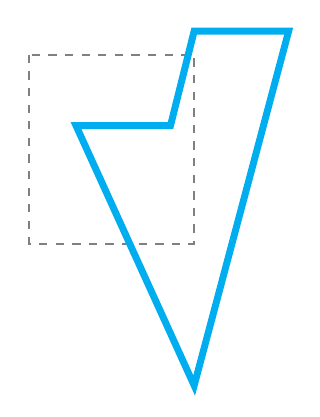
\begin{tikzpicture}[scale=0.3]

\draw[gray, thick, dashed] (4, -1) rectangle (11, -9);

\drawInvertedTriangle{magenta!70}{2.5pt}{10cm}{20cm}{(0,0)}

\begin{scope}

   \coordinate (leftTop) at (6, -4);
   \coordinate (middle) at ([xshift=4cm] leftTop);
   \coordinate (middleTop) at ([xshift=1cm, yshift=4cm] middle);
   \coordinate (rightTop) at ([xshift=4cm] middleTop);
   \coordinate (bottom) at ([yshift=-15cm] middleTop);

   \draw[cyan, line width=2.5pt] (leftTop) -- (middle) -- (middleTop) -- (rightTop) -- (bottom)--  cycle;

\end{scope}
\end{tikzpicture}

      \caption{Общий вид.}
      \label{fig:impossible_config}
    \end{subfigure}
    \hfill
    \begin{subfigure}{0.45\textwidth}
      \centering
      \begin{tikzpicture}[scale=0.7]

\clip (4, -1) rectangle (11, -9);

\node at (9, -1.7) [magenta!70, font=\fontsize{24}{28}\selectfont] {$\alpha$};

\node at (10.15, -1.7) [cyan, font=\fontsize{24}{28}\selectfont] {$\beta$};

\drawInvertedTriangle{magenta!70}{2.5pt}{10cm}{20cm}{(0,0)}

\begin{scope}

   \coordinate (leftTop) at (6, -4);
   \coordinate (middle) at ([xshift=4cm] leftTop);
   \coordinate (middleTop) at ([xshift=1cm, yshift=4cm] middle);
   \coordinate (rightTop) at ([xshift=4cm] middleTop);
   \coordinate (bottom) at ([yshift=-15cm] middleTop);

   \draw[cyan, line width=2.5pt] (leftTop) -- (middle) -- (middleTop) -- (rightTop) -- (bottom)--  cycle;

\end{scope}


\node at (6, 0) (out1) {};
\node at (8, 0) (out2) {};

\node at (6, -8) (out3) {};
\node at (9, -8) (out4) {};

\node[circle, draw=magenta!70, line width=1.5pt, inner sep=0pt, minimum size=0.8cm] at (7,-2.5) [magenta!70, font=\fontsize{20}{28}\selectfont] (first) {1};

\node[circle, draw=cyan, line width=1.5pt, inner sep=0pt, minimum size=0.8cm] at (7.5,-5) [cyan, font=\fontsize{20}{28}\selectfont] (second) {2};

\draw[magenta!70, line width=1.5pt, {Stealth}-] (first) to[bend left] (second);

\draw[magenta!70, dashed, line width=1.5pt] (out1) to (first);
\draw[magenta!70, dashed, line width=1.5pt] (out2) to (first);
, line width=1.5pt
\draw[magenta!70, dashed, line width=1.5pt, {Stealth}-] (second) to (out3);
\draw[cyan, line width=1.5pt, dashed, {Stealth}-] (second) to (out4);


\end{tikzpicture}

      \caption{Относительное расположение вершин.}
      \label{fig:impossible_config_closer_look}
    \end{subfigure}
    \caption{
      Невозможная конфигурация графа состояний.
    }
    \label{fig:all_impossible}
  \end{figure}

  \begin{figure}[htbp]
    \centering
    \begin{subfigure}{0.45\textwidth}
      \centering
      \begin{tikzpicture}
    \drawInvertedTriangle{magenta!70}{2.5pt}{3cm}{4cm}{(0,0)}
    \drawInvertedTriangle{magenta!70}{2.5pt}{3cm}{5cm}{(2,0)}
\end{tikzpicture}

      \caption{Один линейный подпорядок с общим подграфом.}
      \label{fig:one_linext_intersect}
    \end{subfigure}
    \hfill
    \begin{subfigure}{0.45\textwidth}
      \centering
      \input{Dissertation/images/1notinter.tex}
      \caption{Один линейный подпорядок с непересекающимися подграфами.}
      \label{fig:one_linext_notintersect}
    \end{subfigure}

    \vspace{5mm}

    \begin{subfigure}{0.45\textwidth}
      \centering
      \begin{tikzpicture}
    \drawInvertedTriangle{orange}{2.5pt}{3cm}{4cm}{(0,0)}
    \drawInvertedTriangle{cyan}{2.5pt}{3cm}{5cm}{(2,0)}
\end{tikzpicture}

      \caption{Два линейных подпорядка с общим подграфом.}
      \label{fig:two_linext_intersect}
    \end{subfigure}
    \hfill
    \begin{subfigure}{0.45\textwidth}
      \centering
      \input{Dissertation/images/2notinter.tex}
      \caption{Два линейных подпорядка с непересекающимися подграфами.}
      \label{fig:two_linext_notintersect}
    \end{subfigure}

    \caption{
      Возмножные конфигурации графа состояний.
    }
    \label{fig:all_sg_conf}
  \end{figure}

  На рисунке~\ref{fig:all_sg_conf} представлены все возможные
  конфигурации графа состояний.
  На примере одного линейного порядка с
  подграфом~\ref{fig:one_linext_intersect}, можно выделить части с
  подграфом и непересекающиеся части.
  Это общее описание конфигурации линейного порядка.
  В общем случае, можно выделить общую и непересекающуюся части,
  однако могут быть и вырожденные случаи, когда во всём линейном
  порядке исток только один.
  Или, как в случае одного линейного порядка с непересекающимися
  подграфами~\ref{fig:one_linext_notintersect}, общей части вообще нет.

  Такая ситуация возможна, когда, например, в многопоточной программе
  существует несколько кластеров операций, и по
  свойству~\ref{eq:clusters_in_sg}, не существует общего подграфа
  между различными кластерами состояний.
  Это значит, что существуют части частично упорядоченного множества
  не связаны с друг с другом, и с точки зрения эффектов в памяти не
  влияющие друг на друга.
  Такое часто можно наблюдать с мало пересекающимися операциями с памятью.
  Как, например, в тестировании TSOTool\fixme{ref}.

  Если у двух различных линейных порядков есть общая
  часть~\ref{fig:two_linext_intersect}, это является индикатором, что
  в частично упорядоченном множестве основной вклад в зависимость
  между операциями вносят именно упорядоченные операции, а так как
  именно модель памяти определяет строгий порядок между операциями с
  памятью, то в такой конфигурации графа состояний исследуется модель памяти.

  Пример с двумя несвязными линейными
  порядками~\ref{fig:two_linext_notintersect}, наоборот иллюстрирует
  ситуацию со слабо упорядоченными, но сильно пересекающимися
  операциями с памятью.

  Таким образом, конфигурация графа напрямую связана с кластеризацией.
  На примере~\ref{fig:one_linext_intersect} можно выделить один
  кластер операций и один кластер состояний.
  Для рисунка~\ref{fig:one_linext_notintersect} -- два кластера
  операций и два кластера состояний.
  Для рисунка~\ref{fig:two_linext_intersect} -- один кластер операций
  и два кластера состояний.
  Для рисунка~\ref{fig:two_linext_notintersect} нельзя сделать
  однозначные выводы.
  Если различные пути формируются из одних и тех же операций с
  памятью, то в этом случае можно выделить один кластер операций и
  два кластера состояний.
  Если из разных операций с памятью, то можно выделить два кластера
  операций и два кластера состояний.

  Таким образом, все линейные порядки частично упорядоченного
  множества характеризуются кластерами операций и кластерами состояний.

  \subsection{Верификация по кластеру
  состояний}\label{sec:ch2/stategraph-cluster-verification}

  Зададим множество всех кластеров операций: $C = \{C_i\}$.
  Зададим множество всех кластеров состояний для данного кластера
  операций: $S_i = \{C_i^{\pi} \mid \forall \pi \in L_P\}$.
  \begin{definition}
    \label{eq:executed_st_cl}
    Если кластер состояний является подмножеством множества
    маркированных вершин
    $\mathcal{M}$~(см.~определение~\ref{def:mark}), то такой кластер
    состояний будем называть \textbf{маркированным}.
    \begin{equation}
      C_i^\pi \text{ -- маркированный, если } C_i^\pi \subseteq \mathcal{M}
    \end{equation}
  \end{definition}
  Первое условие корректности~\ref{eq:verif-1st} многопоточной
  программы остаётся неизменным.
  Упростим второе условие корректности с учётом введения кластеров
  операций и кластеров состояний.
  Получим кластеризованное условие корректности~\ref{eq:verif-cluster}.

  \textbf{Кластеризованное условие корректности} исполнения
  многопоточной программы: для каждого кластера операций существует
  хотя бы один маркированный кластер состояний.
  \begin{align}
    \label{eq:verif-cluster}
    \text{Исполнение программы корректно, если } \forall S_i \exists
    C_i^\pi \subseteq \mathcal{M}
  \end{align}
  Выполнение этого условия обеспечивает соответствие исполнения
  многопоточной программе заданной модели памяти.

  \begin{lemma}
    Из выполнения условий корректности~\ref{eq:verif-1st}
    и~\ref{eq:verif-cluster} следует выполнение второго условия
    корректности~\ref{eq:verif-2nd}.
    \label{lm:verif-cluster}
  \end{lemma}

  \begin{proof}
    Из выполнения кластеризованного условия корректности следует, что
    $\forall C_i \in C \rightarrow \exists C_i^\pi \in S_i \mid
    C_i^\pi \subseteq \mathcal{M}$.

    Для каждого $C_i$ зафиксируем такой маркированный кластер
    состояний $C_i^\pi$.
    Для него выполняется свойство~\ref{eq:state_cluster_property},
    что все вершины кластера достижимы обходом bfs из истоков этого кластера.

    Таким образом, сформируем множество
    \begin{equation}
      visited = \{ \rho \in C_i^\pi \mid C_i^\pi \text{ --
      маркированный, } \forall C_i \in C \} \\
    \end{equation}

    Для множества $visited$ верно, что $\forall \rho \in visited
    \rightarrow \rho \in \mathcal{M}$, а так как $\bigcup\limits_{C_i
    \in C}{C_i} = P$, то $op(visited) = P$.
    Следовательно верно второе условие корректности.
  \end{proof}

  Таким образом, для проверки корректности выполнения многопоточной
  программы достаточно проверить все кластеры состояний.

  \subsection{Тестовое покрытие. Насыщение}\label{sec:ch2/saturation}

  В тестировании многопоточных систем открытым вопросом является
  тестовое покрытие~\cite{coverage1, coverage2}.
  Достижение полного тестового покрытия всех возможных состояний
  многопроцессорной системы является фундаментально неразрешимой задачей.
  Эта невозможность обусловлена в первую очередь проблемой
  комбинаторного роста числа состояний, когда количество возможных
  конфигураций системы растет экспоненциально с увеличением числа
  компонентов~\cite{formal_verif_tequinique, exp_expl}.
  Если предположить, что каждая из $N$ компонент может находиться в
  $S$ состояниях, то общее количество состояний всей системы составит $S^N$.
  Более того, проблема усугубляется недетерминированностью порядка
  параллельного выполнения.
  Добавление асинхронных событий, таких как доступы в одну память,
  которые могут приходить в любом порядке, приводит к росту числа
  возможных сценариев, эквивалентному факториалу от числа таких
  событий $N!$(см.~\ref{eq:topo-comp-lims}).

  Для решения этой проблемы, для каждого исследумого поведения
  вводится своя анализируемая метрика покрытия.
  В случае с литмус-тестированием~\ref{sec:litmus-intro} определяется
  минимальный набор тестов, который демонстрирует все различия в
  сравниваемых моделях памяти.
  И внутри одного теста, набирается статистика о наблюдаемых
  различных состояниях, как на примере
  \text{SB+rfi-pos.litmus}~\ref{lst:sb-rfi}.
  Тест может исполнятся до тех пор, пока не будет посещено состояние,
  уникальное для данной модели памяти.
  Так как сами тесты небольшие и нацелены на обнаружение конкретного
  эффекта модели памяти, то такой формат статистики согласуется с
  целевым использование инструмента.
  В случае использования инструмента TrekApp~\ref{sec:trekapp} для
  прямого тестирования, тест явно сконфигурирован для приведения
  кэшей в исследуемое состояния.
  И уже покрытие всех состояний кэшей является ответственностью пользователя.
  В инструментах TSOTool~\ref{sec:manovit} и
  Axe~\ref{sec:manovit-adv} не приведена информация о покрытии
  генерируемыми тестами.

  \begin{minipage}{\textwidth}
    \centering
    \lstinputlisting[caption={Гистограма состояний теста
    \text{SB+rfi-pos.litmus}.}, label={lst:sb-rfi}, captionpos=b]{src/sb-rfi.s}
  \end{minipage}

  Во первых, исследуемая в работе модель описания многопоточной
  программы через частично упорядоченное множества из операций с
  памятью, зависит только от модели памяти, что в свою очередь
  сводится к схожести собираемых метрик с литмус-тестированием.
  Во вторых, модель описания многопоточной программы независима от
  конкретных реализаций кэшей и опираций с памятью многопточной
  системы, поэтому нет возможности анализировать покрытие с точки
  зрения состояний кэшей или набора инструкций.

  Введение кластеров операций и кластеров состояний позволяет
  разбивать результат исполнения многопоточной программы на
  независимые исследуемые блоки -- кластеры состояний $C_i^\pi$.
  Во время верификации многопоточной программы по кластеру
  состояний~\ref{sec:ch2/stategraph-cluster-verification}, будем
  отслеживать сколько раз был каждый $C_i^\pi$ был маркированный
  (см.~\ref{eq:executed_st_cl}).
  Операция $cnt(C_i^\pi)$ возвращает это значение.

  Пусть всего многопоточная программа была исполнена $N$ раз.
  Тогда выполнено условиe~\ref{eq:saturation_condi}.
  \begin{equation}
    \forall C_i \in C \rightarrow \sum_{C_i^\pi \in S_i}{cnt(C_i^\pi)} = N
    \label{eq:saturation_condi}
  \end{equation}
  Таким образом, сумма всех маркированных кластеров состояний для
  каждого кластера операций равна общему количеству выполнений программы.
  Добавив информацию о различных конфигурация графа состояний, по
  распределению маркированных кластеров состояний можно сделать
  следующие выводы:
  \begin{itemize}
    \item Если существует только один кластер состояний для данного
      кластера операций: $|S_i| = 1$, то порядок исполнения операций
      данного кластера состояний строго определён.
      Такой случай возможен в строго упорядоченном множестве, или
      если нет никаких пересечений между операциями с памятью.
      Это частый тестовый сценарий, когда необходимо протестировать
      непересекающиеся доступы в память, но которые неявно связаны
      конкретной реализацией тестируемой системы.
      Например, лежат в одной кэш-линии~\cite{false-sharing}  или в
      разных адресных страницах~\cite{page-table}.
    \item Если существует много кластеров состояний для данного
      кластера операций: $|S_i | \gg 1$, то существует множество
      зависимостей между операциями, и по анализу маркированных
      кластеров состояний косвенно можно определить, какие состояния
      были наблюдаемые просто из-за различных порядков зависимых
      операций, а какие состояния могли наблюдаться из-за модели памяти.
      \begin{itemize}
        \item В случае, если количество маркированных кластеров
          состояний равно распределенно: $C_i^\alpha, C_i^\beta \in
          S_i \rightarrow cnt(C_i^\alpha) \approx cnt(C_i^\beta)$, то
          это признак взаимного переупорядочивания зависимых опреций.
        \item Однако если существует такой кластер состояний, который
          был маркирован существенно меньше раз: $\exists C_i^\alpha
          \in S_i \mid \forall C_i^\beta \in S_i \rightarrow
          cnt(C_i^\alpha) \ll cnt(C_i^\beta)$, то
          то это может указывает на эффект модели памяти.
      \end{itemize}
  \end{itemize}

  Так же, благодоря возможности маркировать кластеры состояний, можно
  ввести метрику насыщения~\ref{eq:satur}.
  \begin{definition}
    \textbf{Насыщение} -- отношение количества ненулевых
    маркированных кластеров состояний к общему числу кластеров состояний.

    \begin{equation}
      sat = \frac
      {\sum\limits_{C_i \in C}{\sum\limits_{C_i^\pi \in
      S_i}{sgn(cnt(C_i^\pi))}}}
      {\sum\limits_{C_i \in C}{|S_i|}}
      \label{eq:satur}
    \end{equation}
  \end{definition}

  Когда насыщение достигает единицы $sat = 1$, значит все возможные
  состояния данной многопоточной программы были промаркированны.
  Поэтому значение насыщения можно использовать, как эвристику
  остановки итераций исполнения многопоточной программы, если
  назначение этой программы -- пронаблюдать состояния системы.
  Соответвенно, если $sat = 1$ за первую итерацию исполнения
  программы, значит, либо все операции с памятью в программе строго
  упорядоченны, либо операции никак не взаимодействуют друг с другом.

  \section{Выводы по главе~\ref{sec:ch4}}

  В главе предложена структура данных -- граф состояний
  (определение~\ref{eq:sg_def}),
  позволяющая компактно хранить результаты обхода частично
  упорядоченного множества операций с памятью. В отличие от прямого
  хранения всех линейных порядков, граф состояний сохраняет только
  пути зависимостей для каждой операции, что существенно сокращает
  объём хранимой информации.
  Доказано, что любые две
  различные вершины графа состояний принадлежат разным классам
  эквивалентности (лемма~\ref{lm:path-unique}), что гарантирует
  отсутствие избыточности при хранении состояний.

  Сформулированы два условия корректности исполнения многопоточной
  программы (см.~\ref{eq:verif-1st}~и~\ref{eq:verif-2nd}) на основе
  графа состояний и доказана
  эквивалентность этих условий условию корректности на основе
  линейных порядков (лемма~\ref{lm:verif-equals}), что подтверждает
  корректность предложенного подхода.

  Введено понятие кластеризации графа состояний на основе компонент
  связности графа​.
  Доказано, что элементы разных компонент связности являются
  независимыми (свойства~\ref{eq:clusters_properties}), а
  соответствующие им кластеры состояний не имеют общих рёбер в графе
  состояний. Это свойство позволяет декомпозировать задачу
  верификации на независимые подзадачи.

  Введена метрика насыщения (формула~\ref{eq:satur}) -- отношение
  количества ненулевых маркированных кластеров состояний к общему
  числу кластеров состояний. Показано, что насыщение может быть
  использовано как эвристика остановки итераций исполнения
  многопоточной программы. Анализ распределения маркированных
  кластеров состояний позволяет различать эффекты, обусловленные
  переупорядочиванием зависимых операций, и эффекты, обусловленные
  моделью памяти, что даёт дополнительную информацию для верификации.

  Таким образом, предложенный в главе граф состояний и связанные с
  ним методы кластеризации и анализа насыщения обеспечивают
  компактное представление всех возможных состояний многопоточной
  программы и эффективную верификацию её исполнения на соответствие
  модели памяти. Разработанные подходы позволяют преодолеть
  экспоненциальный рост числа состояний, характерный для прямого
  построения всех линейных порядков, и масштабировать верификацию на
  программы с большим числом операций с памятью.

  \clearpage
